\section{Trabalhos relacionados}

A presente seção tem por finalidade situar a proposta desta pesquisa no contexto da produção científica recente sobre representações neurais de cena, com ênfase em \textit{Neural Radiance Fields} (NeRF), \textit{3D Gaussian Splatting} (3DGS) e aplicações voltadas à síntese de novas vistas, renderização em tempo real e realidade virtual. Mais do que apresentar uma enumeração de estudos correlatos, busca-se estabelecer um posicionamento analítico da pesquisa, evidenciando os avanços do estado da arte, as limitações ainda presentes e a lacuna específica à qual esta investigação se vincula.

Para organizar essa análise, os estudos foram selecionados por meio de um protocolo de revisão com foco aplicado, descrito nas subseções seguintes.

\subsection{Protocolo de busca e seleção dos estudos}

O protocolo adotado delimita o objetivo da revisão, a base de busca, o recorte temporal, o idioma, a string utilizada e os critérios de inclusão e exclusão dos estudos. Com isso, busca-se tornar explícito o processo de seleção das referências analisadas e reduzir a subjetividade da revisão.

\subsection{Objetivo da revisão}

O objetivo da revisão foi identificar e analisar estudos que contribuam para a compreensão das seguintes dimensões do problema:

\begin{itemize}
    \item fundamentos das representações implícitas baseadas em NeRF;
    \item técnicas de aceleração da reconstrução e da renderização neural;
    \item alternativas explícitas voltadas ao desempenho em tempo real;
    \item estudos que tratem da adaptação dessas representações ao contexto de realidade virtual;
    \item trabalhos que discutam integração com motores gráficos e ambientes de execução interativos.
\end{itemize}

A revisão foi orientada, portanto, pela seguinte questão de pesquisa:

\begin{quote}
\textit{De que maneira os estudos recentes sobre NeRF e 3D Gaussian Splatting enfrentam o compromisso entre qualidade visual, desempenho computacional e adequação ao uso em aplicações de realidade virtual?}
\end{quote}

\subsection{Base de busca, recorte temporal e idioma}

Como base principal de busca, foi adotado o Google Scholar, em razão de sua abrangência na indexação de artigos de periódicos, anais de conferências e publicações amplamente reconhecidas na área de Computação Gráfica, Visão Computacional e Realidade Virtual. Tal escolha também se mostrou coerente com a orientação de priorizar estudos consolidados e evitar a dependência de versões preliminares disponibilizadas apenas como \textit{preprints}.

O recorte temporal considerado compreende o período de 2020 a 2025. A escolha desse intervalo decorre do fato de que o trabalho seminal sobre NeRF foi publicado em 2020, inaugurando uma nova fase de intensa produção científica em torno de representações neurais para síntese de vistas. A partir de 2023, com a publicação do 3D Gaussian Splatting, observa-se uma inflexão importante na literatura, marcada pela valorização de representações explícitas orientadas ao desempenho em tempo real. O idioma prioritariamente considerado foi o inglês, por concentrar os principais veículos científicos da área.

\subsection{String de busca}

A estratégia de busca foi estruturada a partir de operadores booleanos,
combinando os principais descritores associados ao problema investigado. Uma
forma representativa da string empregada é apresentada a seguir:

\begingroup
\shorthandoff{"}
\begin{quote}
\ttfamily\raggedright
("Neural Radiance Fields" OR NeRF OR "3D Gaussian Splatting") AND ("virtual reality" OR VR OR "real-time rendering" OR "walkable spaces" OR "Unreal Engine")
\end{quote}
\endgroup

Em buscas complementares, foram utilizados termos adicionais, como \texttt{"scene \newline reconstruction"}, \texttt{"novel view synthesis"} e \texttt{"immersive rendering"}, \\ com o objetivo de refinar os resultados e ampliar a aderência ao escopo da pesquisa.

\subsection{Critérios de inclusão e exclusão}

Foram definidos os seguintes critérios de inclusão:

\begin{itemize}
    \item estudos publicados em periódicos ou anais de conferências reconhecidos na área;
    \item estudos publicados entre 2020 e 2025;
    \item pesquisas diretamente associadas a NeRF, 3DGS, reconstrução de cenas, síntese de novas vistas, renderização em tempo real ou realidade virtual;
    \item estudos que apresentem contribuição conceitual, metodológica ou aplicada relevante para o problema de pesquisa do presente trabalho.
\end{itemize}

Por sua vez, os critérios de exclusão foram:

\begin{itemize}
    \item estudos disponíveis apenas em versões preliminares, sem publicação formal consolidada;
    \item estudos sem aderência direta ao tema de reconstrução de cenas e visualização imersiva;
    \item publicações duplicadas ou versões redundantes de um mesmo trabalho;
    \item artigos cujo foco principal se situe em problemas periféricos ao escopo desta pesquisa.
\end{itemize}

\section{Discussão dos estudos selecionados}

Esta seção discute os estudos selecionados, destacando suas principais contribuições, limitações e relações com o \textit{pipeline} proposto nesta pesquisa.

\subsection{\textit{NeRF: Representing Scenes as Neural Radiance Fields for View Synthesis}}

O trabalho de Mildenhall et al. \cite{mildenhall2020} constitui o marco fundador da linha contemporânea de pesquisa em campos neurais para síntese de novas vistas.

Sua principal contribuição está na formulação de uma representação implícita contínua da cena, parametrizada por uma rede neural do tipo \textit{multilayer perceptron} (MLP), que recebe como entrada uma coordenada espacial tridimensional e uma direção de observação, produzindo como saída a densidade volumétrica e a cor correspondente naquele ponto. A imagem final é obtida por integração ao longo dos raios emitidos pela câmera, em um processo de renderização volumétrica diferenciável.

A Figura \ref{fig:nerf_esquema} é especialmente elucidativa porque condensa, em um único diagrama, o núcleo conceitual do método. Observa-se que o modelo não aprende diretamente uma malha, uma nuvem de pontos ou uma textura, mas sim uma função contínua que associa amostras espaciais a propriedades radiométricas. Esse aspecto é decisivo para compreender tanto a capacidade do NeRF de produzir vistas fotorealistas quanto seu custo computacional: como a imagem precisa ser composta a partir de múltiplas amostras por raio, a elevada fidelidade visual vem acompanhada de um processo de inferência oneroso.

\begin{figure}[H]
    \centering
    \fbox{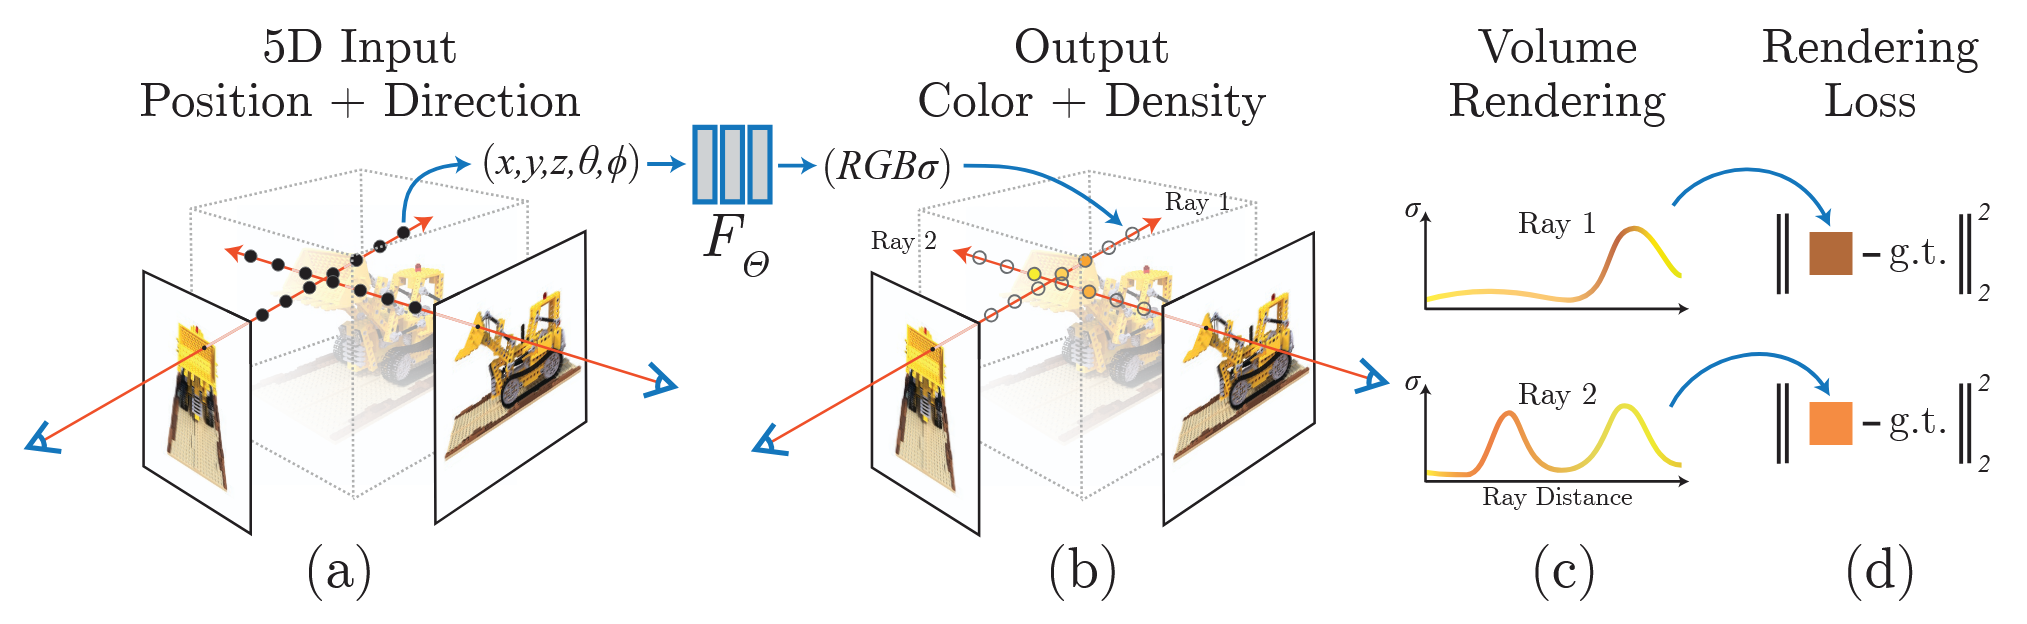
\includegraphics[width=0.92\textwidth]{figuras/mildenhall2020_fig2.png}}
    \caption{Representação esquemática do NeRF. A figura mostra a entrada 5D composta por posição e direção de observação, o mapeamento por uma MLP para cor e densidade e, por fim, a integração volumétrica ao longo dos raios. Fonte: \cite{mildenhall2020}.}
    \label{fig:nerf_esquema}
\end{figure}

Essa formulação foi decisiva porque rompeu com abordagens anteriores baseadas em discretizações rígidas, voxels densos ou estruturas explícitas de custo elevado, oferecendo uma representação compacta e contínua, capaz de modelar efeitos dependentes da direção de observação e detalhes geométricos complexos. O artigo demonstra que, a partir de um conjunto relativamente esparso de imagens com poses conhecidas, é possível sintetizar novas vistas com alto grau de fotorrealismo e consistência multivista.

Para a presente pesquisa, este trabalho é central porque estabelece o referencial teórico a partir do qual se desenvolvem tanto as técnicas de aceleração quanto as alternativas explícitas posteriormente discutidas. Ao mesmo tempo, ele explicita uma limitação estrutural importante: a elevada demanda computacional associada ao treinamento e, sobretudo, à renderização baseada em amostragem volumétrica ao longo dos raios. Em consequência, embora o NeRF apresente notável qualidade de reconstrução e síntese, sua aplicação direta em ambientes imersivos em tempo real permanece restrita.

\subsection{\textit{Instant Neural Graphics Primitives with a Multiresolution Hash Encoding}}

Müller et al. \cite{muller2022} propõem uma contribuição decisiva para a viabilidade prática das representações neurais ao introduzir uma estratégia de codificação multirresolução baseada em tabelas hash treináveis. Em vez de depositar toda a capacidade representacional em uma MLP relativamente grande, o método distribui uma parte significativa da descrição espacial da cena em uma estrutura hierárquica de características indexadas de forma eficiente, permitindo o uso de redes menores e uma inferência mais rápida.

A Figura \ref{fig:instantngp_encoding} é particularmente relevante porque não se limita a ilustrar o método, mas demonstra empiricamente por que a codificação proposta se tornou tão influente. A comparação mostra que abordagens sem codificação ou com codificações convencionais tendem a produzir resultados mais borrados ou a exigir estruturas muito mais pesadas. Em contrapartida, a tabela hash multirresolução apresentada pelos autores preserva detalhes finos com um custo computacional mais favorável. Assim, a imagem sustenta visualmente o argumento central do artigo: ganhos expressivos de eficiência podem ser obtidos por meio da representação dos dados, e não apenas pelo aumento da capacidade da rede.

\begin{figure}[H]
    \centering
    \fbox{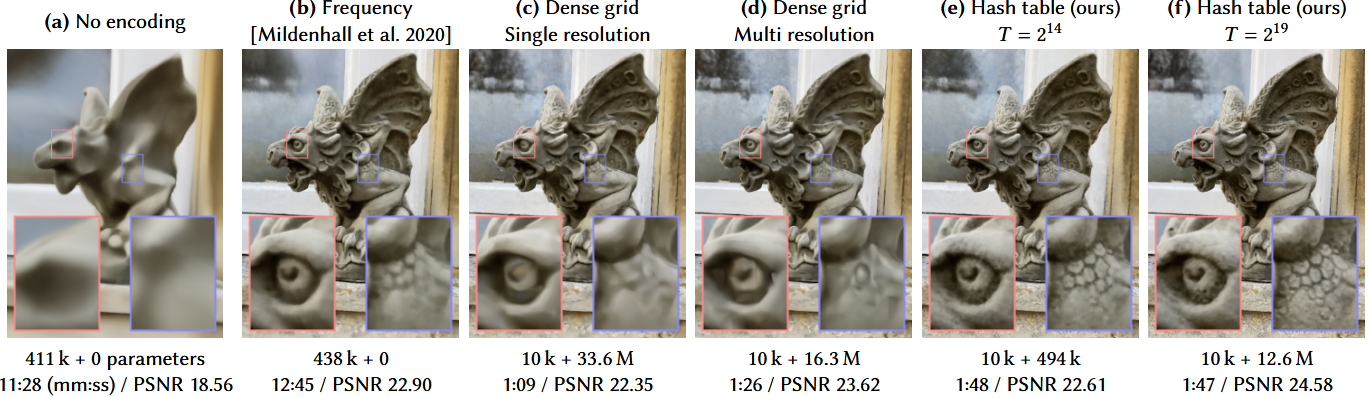
\includegraphics[width=0.95\textwidth]{figuras/muller_fig2.png}}
    \caption{Comparação entre diferentes estratégias de codificação no Instant-NGP. A figura evidencia o compromisso entre número de parâmetros, tempo de treinamento e qualidade visual, destacando o desempenho da codificação por tabela hash multirresolução. Fonte: \cite{muller2022}.}
    \label{fig:instantngp_encoding}
\end{figure}

O avanço apresentado por esse trabalho é particularmente relevante porque atenua uma das principais restrições do NeRF original: o elevado custo de otimização. Ao reduzir drasticamente o tempo necessário para treinamento, o Instant-NGP reposiciona os campos neurais como ferramentas mais acessíveis em contextos experimentais, prototipagem rápida e reconstrução iterativa. Além disso, o método também evidencia que ganhos substanciais de desempenho podem ser obtidos não apenas por mudanças na formulação do modelo, mas sobretudo por escolhas de representação e implementação fortemente alinhadas à arquitetura de hardware disponível.

No contexto desta pesquisa, a relevância do Instant-NGP reside em funcionar como elo intermediário entre a formulação original do NeRF e os esforços posteriores de aproximação ao tempo real. O artigo não elimina integralmente os obstáculos à adoção em realidade virtual, mas demonstra que a fronteira entre qualidade visual e viabilidade computacional é mais flexível do que sugeria a formulação inicial dos campos neurais. Isso é particularmente importante para um trabalho que busca avaliar a aplicabilidade de técnicas neurais em um \textit{pipeline} orientado à visualização imersiva.

Outro aspecto relevante é que o Instant-NGP influenciou diretamente trabalhos posteriores voltados à captura e renderização de cenas complexas, inclusive em contextos de alta resolução e amplo alcance espacial. Assim, mais do que uma técnica de aceleração isolada, o artigo representa uma mudança de perspectiva: ele mostra que a discussão sobre representações neurais de cena deve considerar, simultaneamente, a formulação matemática, a estrutura de dados e a eficiência de execução.

\subsection{\textit{VR-NeRF: High-Fidelity Virtualized Walkable Spaces}}

Xu et al. \cite{xu2023} apresenta um dos trabalhos mais próximos do problema investigado nesta pesquisa, ao propor um sistema de ponta a ponta para captura, reconstrução e visualização de espaços caminháveis em realidade virtual. A contribuição do estudo não se limita à modelagem da cena, mas abrange todo o \textit{pipeline}, desde a aquisição de imagens em alta resolução e alta faixa dinâmica até a renderização em tempo compatível com uma experiência imersiva. Esse caráter sistêmico torna o trabalho particularmente relevante, pois aproxima a discussão acadêmica de um cenário de uso efetivo.

A Figura \ref{fig:vrnerf_overview} evidencia o caráter sistêmico da proposta. Diferentemente de trabalhos centrados apenas na síntese de novas vistas em visualização convencional, o VR-NeRF articula captura especializada, modelagem adaptada e renderização binocular, deixando claro que o problema em VR não se resume à qualidade da reconstrução. A imagem também é relevante por mostrar que os autores tratam explicitamente componentes auxiliares, como profundidade, normais, níveis de detalhe e grade de ocupação, indicando uma preocupação com eficiência e estabilidade visual além da simples reprodução fotográfica.

\begin{figure}[H]
    \centering
    \fbox{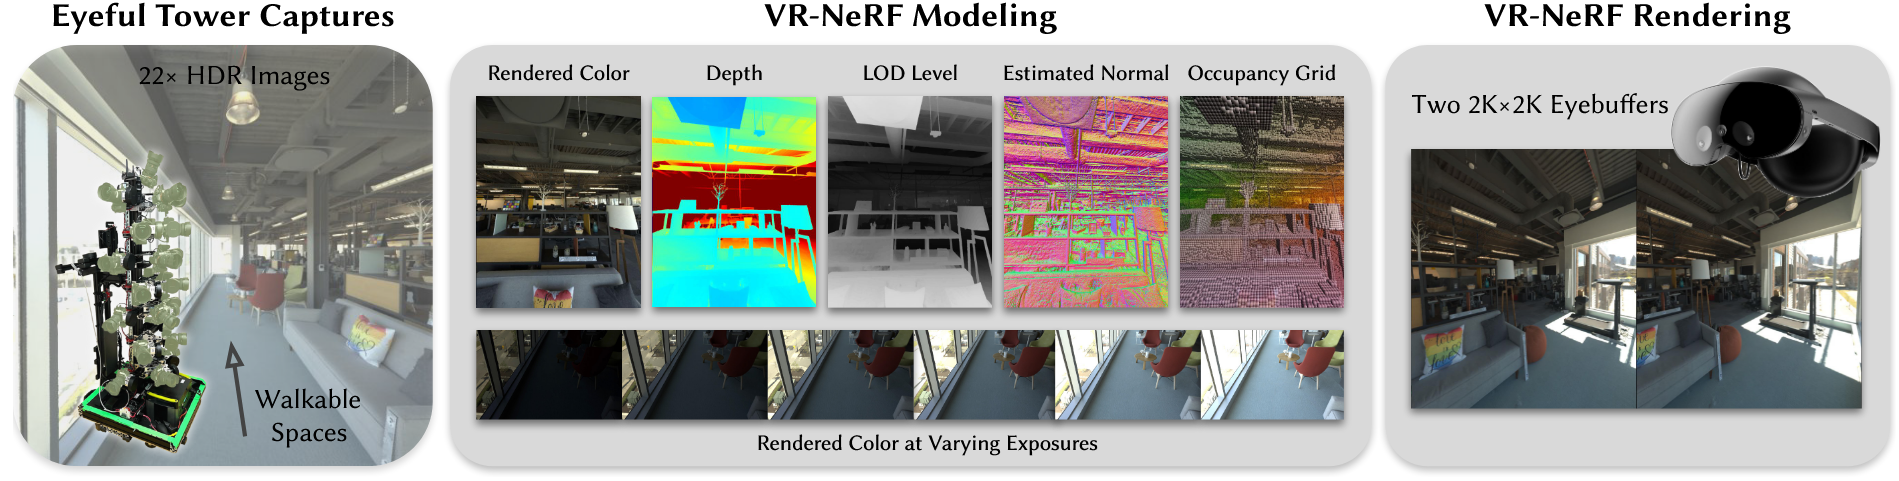
\includegraphics[width=0.98\textwidth]{figuras/xu_2023_fig1.png}}
    \caption{Visão geral do sistema VR-NeRF, contemplando captura, modelagem da cena e renderização em \textit{eyebuffers} binoculares para realidade virtual. Fonte: \cite{xu2023}.}
    \label{fig:vrnerf_overview}
\end{figure}

Um dos diferenciais centrais do VR-NeRF é a preocupação com limitações específicas da realidade virtual. Em vez de tratar o problema apenas como síntese de novas vistas, os autores consideram exigências como liberdade de exploração espacial, estabilidade visual, alta resolução binocular, preservação de detalhes finos e compatibilidade com renderização interativa. Para isso, o trabalho combina adaptações na linha do Instant-NGP, como tratamento mais adequado de imagens HDR, mecanismos de \textit{level of detail} e estratégias de renderização multi-GPU.

A Figura \ref{fig:vrnerf_scaling} complementa a discussão ao tornar visível um dos pontos mais importantes do artigo: a dependência de infraestrutura robusta para alcançar desempenho compatível com VR. As curvas mostram que a taxa de quadros cresce com o número de GPUs, enquanto as linhas de referência tornam explícitos os patamares de desempenho almejados. Em termos analíticos, essa imagem é
fundamental porque reforça uma conclusão importante para a presente pesquisa: o VR-NeRF demonstra a viabilidade técnica da abordagem implícita, mas essa viabilidade ainda se apoia em um orçamento computacional elevado.

\begin{figure}[H]
    \centering
    \fbox{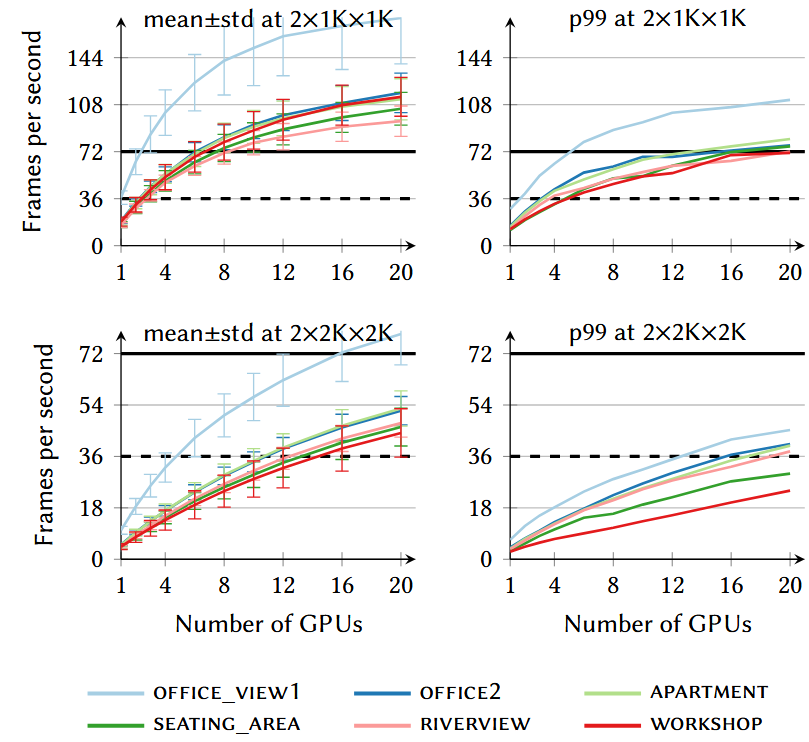
\includegraphics[width=0.72\textwidth]{figuras/xu_2023_fig3.png}}
    \caption{Escalabilidade do VR-NeRF em função do número de GPUs, com indicação dos patamares de desempenho associados à renderização imersiva em diferentes resoluções binoculares. Fonte: \cite{xu2023}.}
    \label{fig:vrnerf_scaling}
\end{figure}

Para o presente trabalho, essa dualidade é especialmente importante. O VR-NeRF funciona como prova de conceito de que campos neurais podem, em condições apropriadas, sustentar experiências imersivas de alta fidelidade. Contudo, também expõe a necessidade de investigar soluções mais pragmáticas, seja por meio de representações mais leves, seja pela conversão para estruturas explícitas mais compatíveis com a renderização em tempo real. Dessa forma, o artigo serve como referência de alto nível para delimitar tanto o potencial quanto as limitações da linha implícita em aplicações de VR.

\subsection{\textit{3D Gaussian Splatting for Real-Time Radiance Field Rendering}}

Kerbl et al. \cite{kerbl2023} introduzem o 3D Gaussian Splatting como uma alternativa explícita aos campos neurais implícitos para a síntese de novas vistas e renderização de campos radiantes. O método parte de uma nuvem inicial de pontos obtida por calibração e estrutura a cena como um conjunto de gaussianas 3D anisotrópicas, cada uma dotada de posição, covariância, opacidade e atributos de aparência. A renderização é realizada por meio de uma rasterização diferenciável e \textit{visibility-aware}, com composição ordenada das contribuições na imagem.

A Figura \ref{fig:3dgs_pipeline} é particularmente útil porque explicita a principal mudança de paradigma introduzida pelo método. Em vez de amostrar densamente ao longo de cada raio, como em abordagens implícitas, o 3DGS projeta gaussianas explicitamente representadas e as compõe de forma eficiente na imagem final. Além disso, o bloco de controle adaptativo de densidade mostra que a representação não é fixa: ela pode ser refinada ao longo da otimização, com clonagem, divisão ou remoção de gaussianas, conforme a complexidade local da cena. Esse ponto ajuda a compreender por que o método consegue combinar boa qualidade visual com alta taxa de renderização.

\begin{figure}[H]
    \centering
    \fbox{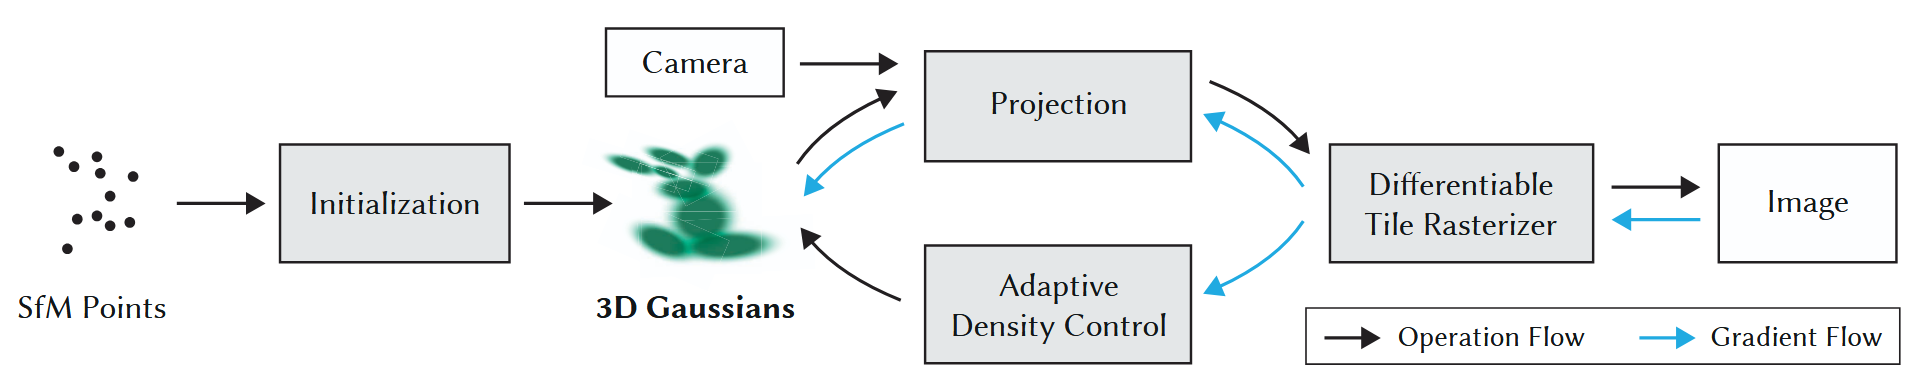
\includegraphics[width=0.92\textwidth]{figuras/kerbl2023_fig2.png}}
    \caption{Esquema do \textit{pipeline} do 3D Gaussian Splatting, incluindo inicialização a partir de pontos de SfM, projeção, rasterização diferenciável e controle adaptativo de densidade. Fonte: \cite{kerbl2023}.}
    \label{fig:3dgs_pipeline}
\end{figure}

A Figura \ref{fig:3dgs_comparison} reforça empiricamente esse reposicionamento do problema. A comparação evidencia que o método proposto pelos autores busca ocupar um ponto intermediário particularmente valioso para aplicações interativas: mantém uma qualidade visual elevada, ao mesmo tempo em que alcança taxas de renderização muito superiores às de abordagens implícitas de maior custo. Nesse sentido, a imagem não funciona apenas como ilustração de resultado, mas como síntese visual da principal tese do artigo: a representação explícita pode reformular de maneira favorável o equilíbrio entre fidelidade e desempenho.

\begin{figure}[H]
    \centering
    \fbox{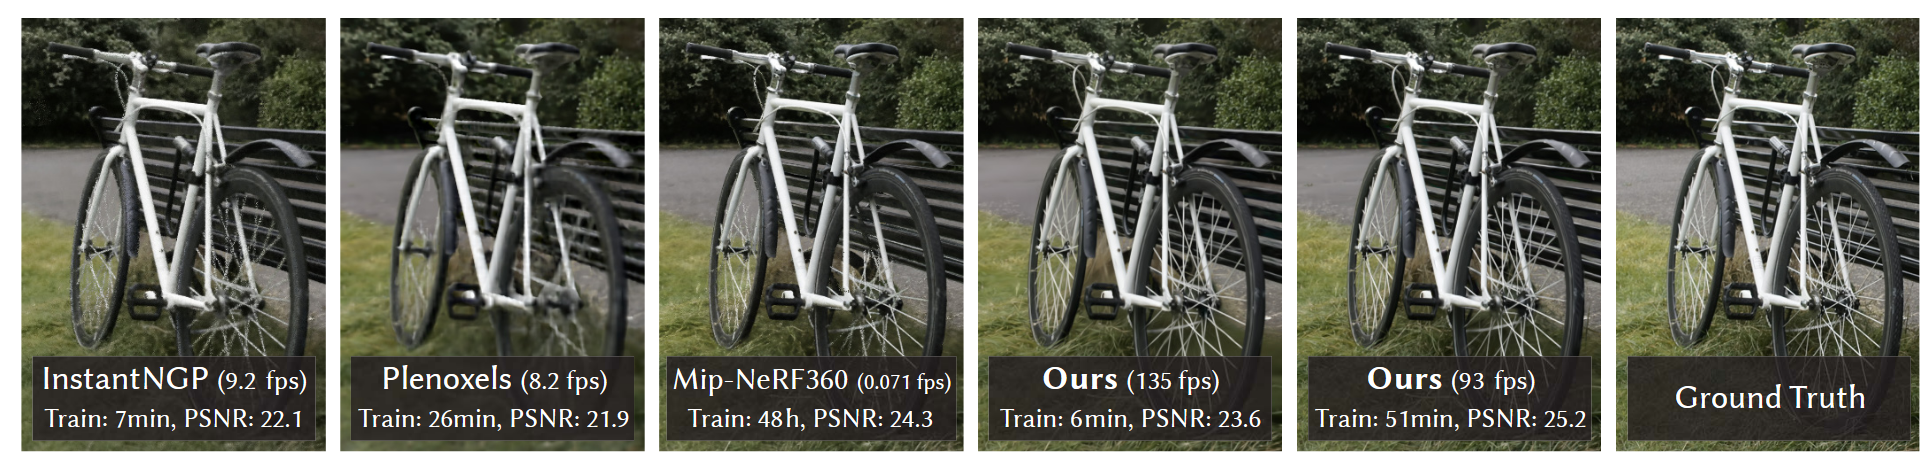
\includegraphics[width=0.97\textwidth]{figuras/kerbl2023_fig1.png}}
    \caption{Comparação visual e de desempenho entre métodos de síntese de novas vistas, evidenciando o compromisso entre tempo de treinamento, taxa de quadros e fidelidade visual. Fonte: \cite{kerbl2023}.}
    \label{fig:3dgs_comparison}
\end{figure}

No escopo desta pesquisa, o trabalho de Kerbl et al. é decisivo por tornar plausível uma estratégia de visualização mais aderente às restrições da realidade virtual. Embora o artigo não resolva, isoladamente, todos os desafios da implantação em ambientes imersivos, ele fornece a base metodológica mais forte para o uso de representações explícitas em cenários nos quais latência, taxa de quadros e previsibilidade de execução assumem um papel central.

\subsection{\textit{UE-GS: High-Quality 3D Gaussian Splatting Real-Time Rendering for Unreal Engine}}

Jin et al. \cite{jin2024} deslocam a discussão do nível estritamente algorítmico para o da integração prática em motor gráfico, ao abordar a renderização 3D Gaussian Splatting no Unreal Engine. Essa mudança de enfoque é altamente relevante para a presente pesquisa, pois o problema investigado não se encerra na capacidade de reconstruir ou sintetizar vistas de uma cena, mas se estende à implantação dessa representação em um ambiente real de desenvolvimento imersivo.

A Figura \ref{fig:uegs_qualitative} é pertinente porque evidencia o tipo de ganho que se torna especialmente relevante em motores gráficos: preservação de contornos, estruturas finas e detalhes locais que costumam se degradar quando a representação não está suficientemente bem integrada ao \textit{pipeline} de renderização. As ampliações em vermelho tornam a comparação mais objetiva, mostrando que a proposta dos autores se aproxima mais da referência do que a renderização 3D-GS tomada como base. Assim, a figura contribui para sustentar o argumento de que a discussão sobre representação de cena precisa ser acompanhada pela discussão sobre implantação em \textit{engine}.

\begin{figure}[H]
    \centering
    \fbox{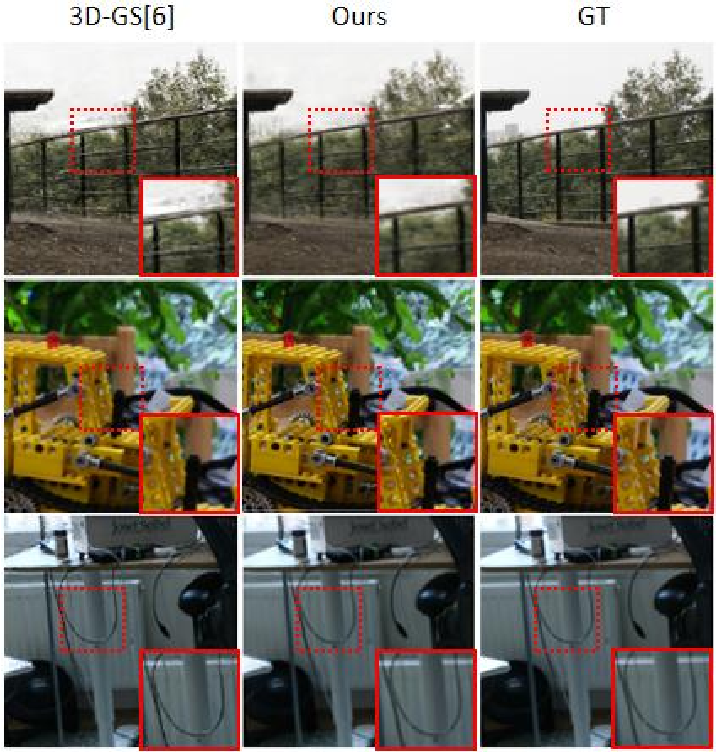
\includegraphics[width=0.50\textwidth]{figuras/jin2025_fig1.png}}
    \caption{Comparação qualitativa entre 3D-GS, a proposta de UE-GS e a imagem de referência, com ampliações destacando detalhes finos. Fonte: \cite{jin2024}.}
    \label{fig:uegs_qualitative}
\end{figure}

A principal pertinência do estudo decorre do fato de que motores gráficos como o Unreal Engine ocupam posição central na produção de experiências interativas, aplicações de visualização e ambientes virtuais. Assim, a integração do 3DGS à \textit{engine} constitui um passo importante na direção de \textit{pipelines} mais aplicáveis, em que a representação da cena não é apenas avaliada por métricas de qualidade de imagem, mas também por sua compatibilidade com ferramentas, rotinas de renderização e mecanismos de interação amplamente utilizados.

Ainda que o trabalho não se concentre especificamente na avaliação de conforto visual ou desempenho em dispositivos autônomos de VR, sua contribuição é metodologicamente significativa. Ele aproxima a literatura de representação neural da dimensão de implantação, aspecto particularmente importante para uma pesquisa cujo objetivo não é apenas compreender o estado da arte, mas examinar sua viabilidade prática em um fluxo de trabalho orientado à realidade virtual.

\subsection{\textit{VRSplat: Fast and Robust Gaussian Splatting for Virtual Reality}}

Tu et al. \cite{tu2025} apresentam um estudo tratando diretamente da adaptação de 3D Gaussian Splatting ao contexto da realidade virtual. Diferentemente de trabalhos que demonstram elevado desempenho apenas em visualização convencional, o VRSplat parte do reconhecimento de que a VR impõe exigências adicionais, como grande campo de visão, renderização estereoscópica, movimentos contínuos de cabeça e tolerância muito menor a artefatos temporais e inconsistências geométricas.

A Figura \ref{fig:vrsplat_pipeline} é particularmente relevante porque sintetiza a principal contribuição metodológica do VRSplat. Em vez de propor uma alteração pontual sobre o 3D Gaussian Splatting, o trabalho organiza um \textit{pipeline} integrado para realidade virtual, partindo de um modelo base eficiente, seguido de uma etapa de \textit{fine-tuning} com rasterização diferenciável livre de artefatos, até chegar a uma etapa de renderização com rasterização foveada. A figura evidencia, portanto, que a proposta dos autores não se limita à melhoria de qualidade visual isolada, mas busca conciliar robustez perceptual e desempenho compatível com aplicações imersivas.

\begin{figure}[H]
    \centering
    \fbox{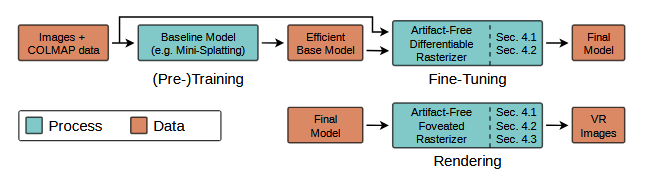
\includegraphics[width=0.80\textwidth]{figuras/tu2025_fig1.png}}
    \caption{Visão geral do pipeline do VRSplat para renderização de alta fidelidade
    em realidade virtual, incluindo modelo base eficiente, etapa de fine-tuning com
    rasterização livre de artefatos e renderização foveada. Fonte: \cite{tu2025}.}
    \label{fig:vrsplat_pipeline}
\end{figure}

Essa combinação evidencia uma mudança de maturidade da área: a discussão deixa de ser apenas “é possível renderizar rápido?” e passa a incorporar “é possível renderizar de forma estável e confortável em VR?”.

Para o presente trabalho, a principal contribuição do VRSplat está em mostrar que o uso de 3DGS em ambientes imersivos exige adaptações específicas, e não uma mera transposição direta de um método originalmente pensado para visualização monocular convencional. Essa observação é essencial, pois reforça a necessidade de que a avaliação experimental considere, além de PSNR, SSIM, LPIPS e FPS, aspectos qualitativos ligados à estabilidade visual e à robustez perceptual.

\section{Quadro comparativo dos estudos}

O Quadro \ref{qua:comparativo_estudos} sintetiza, de forma objetiva, as principais características dos estudos selecionados, com ênfase no tipo de representação adotada, no foco metodológico, na forma de avaliação dos resultados, nos dados ou cenários utilizados e nas limitações mais relevantes frente ao problema investigado. A análise detalhada de cada estudo é apresentada ao longo da seção, enquanto o quadro busca apenas explicitar, de maneira resumida, os principais pontos de convergência e distinção.

\begin{quadro}[H]
\centering
\footnotesize
\caption{Quadro comparativo dos estudos selecionados.}
\label{qua:comparativo_estudos}
\renewcommand{\arraystretch}{1.15}
\setlength{\tabcolsep}{3pt}
\begin{tabularx}{\textwidth}{|p{2.5cm}|p{2.5cm}|p{1.8cm}|p{2.3cm}|p{2.6cm}|X|}
\hline
\textbf{Estudo} & \textbf{Representação} & \textbf{Ênfase} & \textbf{Avaliação dos resultados} & \textbf{Dados/cenários utilizados} & \textbf{Limitação} \\
\hline

\textit{NeRF} \cite{mildenhall2020}
& Implícita
& Fidelidade
& PSNR, SSIM, visual
& Cenas sintéticas e reais
& Alto custo computacional \\
\hline

\textit{Instant-NGP} \cite{muller2022}
& Implícita
& Aceleração
& Qualidade e tempo
& Cenas variadas
& VR não tratada diretamente \\
\hline

\textit{VR-NeRF} \cite{xu2023}
& Implícita
& VR
& Fidelidade e FPS
& Ambientes capturados
& Dependência de multi-GPU \\
\hline

\textit{3D Gaussian Splatting} \cite{kerbl2023}
& Explícita
& Tempo real
& PSNR, SSIM, LPIPS, FPS
& Mip-NeRF360, Tanks and Temples, Deep Blending
& VR não abordada diretamente \\
\hline

\textit{UE-GS} \cite{jin2024}
& Explícita
& Engine
& Comparação visual e FPS
& Cenas integradas à engine
& VR autônoma ausente \\
\hline

\textit{VRSplat} \cite{tu2025}
& Explícita
& VR
& FPS, visual, estudo com usuários
& Cenas para VR
& Solução específica para 3DGS \\
\hline

\end{tabularx}
\end{quadro}

A análise sintetizada no Quadro \ref{qua:comparativo_estudos} evidencia, em primeiro lugar, uma transição metodológica importante no campo das representações neurais de cena. O trabalho de Mildenhall et al. \cite{mildenhall2020} estabelece a base conceitual das representações implícitas, demonstrando elevada capacidade de síntese de novas vistas, porém à custa de alto esforço computacional. Em seguida, Müller et al. \cite{muller2022} mostram que esse custo pode ser reduzido de forma significativa por meio de estratégias mais eficientes de codificação, tornando os campos neurais mais viáveis em contextos experimentais.

No recorte específico da realidade virtual, Xu et al. \cite{xu2023} representam um marco relevante ao demonstrarem que campos neurais podem ser empregados na captura, modelagem e visualização de espaços caminháveis com elevado grau de fidelidade. Entretanto, o estudo também evidencia que essa viabilidade depende de infraestrutura robusta, especialmente em termos de aquisição de dados e processamento multi-GPU. Em outras palavras, o VR-NeRF confirma o potencial científico da abordagem implícita em VR, mas também explicita os obstáculos práticos associados à sua adoção em cenários mais acessíveis.

Por outro lado, os estudos baseados em 3D Gaussian Splatting apontam uma mudança de ênfase em direção a representações explícitas mais compatíveis com
renderização eficiente. Kerbl et al. \cite{kerbl2023} reposicionam o debate ao mostrar que é possível obter elevada qualidade visual com taxas de renderização substancialmente mais adequadas ao tempo real. Jin et al. \cite{jin2024}, ao aproximarem essa representação do Unreal Engine, reforçam a importância da implantação em motores gráficos reais, enquanto Tu et al. \cite{tu2025} avançam na adaptação desse paradigma às exigências específicas da realidade virtual, como robustez perceptual, mitigação de artefatos e desempenho compatível com uso imersivo.

A inclusão das colunas referentes à avaliação dos resultados e aos dados ou cenários utilizados permite observar que os estudos não diferem apenas em sua formulação metodológica, mas também na forma como validam suas contribuições. Enquanto alguns trabalhos se apoiam predominantemente em métricas objetivas de qualidade e desempenho, outros incorporam comparações visuais, cenários capturados em ambiente real e até avaliações perceptuais com usuários. Essa distinção é particularmente relevante porque evidencia que, no contexto da realidade virtual, a análise de resultados não pode se restringir apenas à fidelidade de reconstrução, devendo também considerar estabilidade visual, robustez perceptual e viabilidade de execução.

Em conjunto, esses estudos mostram que a literatura evoluiu de modelos fortemente orientados à fidelidade visual para soluções cada vez mais comprometidas com viabilidade prática, integração e desempenho. Contudo, também revelam que ainda persiste uma lacuna entre a excelência técnica dos métodos propostos e sua adoção em um fluxo de trabalho aplicado, capaz de articular reconstrução neural, representação eficiente da cena e uso em realidade virtual sob restrições concretas de hardware e execução.

É nesse contexto que se insere o presente trabalho. Em vez de se restringir à análise isolada de uma única técnica, esta pesquisa propõe uma abordagem aplicada, voltada à avaliação da viabilidade de um \textit{pipeline} que envolva reconstrução neural, representação eficiente e integração em ambiente imersivo. Desse modo, busca-se compreender, de forma experimental, em que medida os avanços observados na literatura podem ser articulados de maneira coerente para atender simultaneamente aos requisitos de qualidade visual, desempenho e implantação prática em realidade virtual.
